\documentclass{article}
\usepackage[margin=0.5in]{geometry}
\usepackage{amsmath}
\usepackage{graphicx}
\usepackage{amssymb}
\usepackage{multicol}
\usepackage{xcolor}
\usepackage{amsthm}
\usepackage{mdframed}

\newenvironment{tightcenter}{%
    \setlength\topsep{0pt}
    \setlength\parskip{0pt}
    \begin{center}
}{%  
    \end{center}
}
\newcommand{\R}{\mathbb{R}}
\newcommand{\C}{\mathbb{C}}
\newcommand{\PP}{\mathbb{P}}
\title{Trabajo Práctico 1 - Repaso }
\author{Santiago}
\date{}
\begin{document}
    \maketitle
    \global\mdfdefinestyle{s}{%
            linecolor=orange,linewidth=0.5pt,%
            leftmargin=0cm,rightmargin=1cm
        }
    \begin{enumerate}
        \item Analizar si los siguientes conjuntos son espacios vectoriales sobre $\R$ ($\R$-EV) con las operaciones + y $\cdot$ usuales.
    \begin{enumerate}
        \item Los puntos de una recta de $\R^2$ que pasa por el origen de coordenadas.
            \begin{mdframed}[style=s]
                Los puntos $s$ que pertenecen a dicha recta son de la forma $s=(x,mx)=x(1,m)$ para algún $m$ arbitrario. Con lo cual, el conjunto de puntos lo podemos denotar $S=\overline{\{(1,m)\}}$. En la Figura 1 se observan varios conjuntos de puntos que cumplen con dicha condición. Es claro que $S$ es un subconjunto de $\R^2$ (el cual es un $\R$-espacio vectorial) y se dice que un subconjunto $S$ es un subespacio de $\R^2$ si se cumple:
                \begin{enumerate}
                    \item $\vec{0}\in S$
                    \item si $s_1,s_2 \in S$, luego $s_1+s_2\in S$
                    \item si $s\in S$ y $\lambda \in \mathbb{K} \to \lambda \cdot s \in S$
                \end{enumerate}
                \begin{center}
                    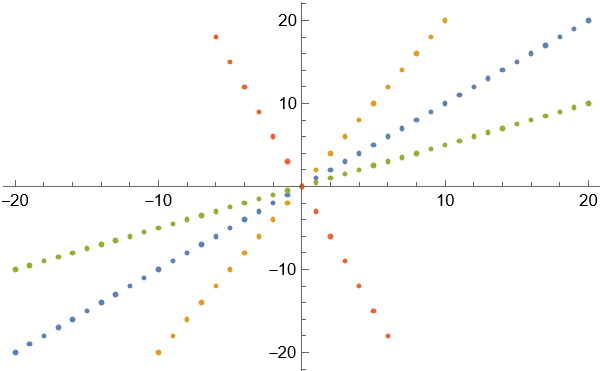
\includegraphics[width=0.4\textwidth]{Ej1a.png}\\
                    Figura 1. Puntos pertenecientes a distintas rectas que incluyen el origen.
                \end{center}
                Además, todo subespacio de un $\R$-espacio vectorial es un $\R$-espacio vectorial.
                \begin{enumerate}
                    \item El $(0,0)=\vec{0}\in S$ ya que la recta pasa por el origen de coordenadas.
                    \item Dados $s_1,s_2\in S, s_1=\alpha(1,m), s_2=\beta(1,m)\to s_1+s_2=\alpha(1,m)+\beta(1,m)=(\alpha + \beta)(1,m)\in S$
                    \item Dados $s\in S, \lambda \in \R, s=\alpha(1,m)\to \lambda s=\lambda\alpha(1,m)=(\lambda\alpha)(1,m)\in S$
                \end{enumerate}
                Como se cumplen las tres condiciones, $S$ es un $\R$-espacio vectorial.
            \end{mdframed}
        \item Las funciones lineales cuya gráfica pertenece a $\R^2$ y contiene al origen de coordenadas.
            \begin{mdframed}[style=s]
                En este caso el conjunto con el que se está tratando es $S=\{f\in \PP_1[x]:f(x)=mx, m\in\R\}$ (Figura 2). Se sabe que el conjunto $\PP_1[x]$ es un espacio vectorial así que como en el caso anterior se verificará que $S$ sea un subespacio.
                \begin{center}
                    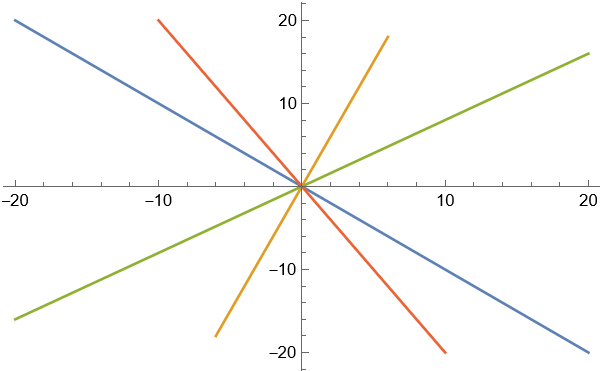
\includegraphics[width=0.4\textwidth]{Ej1b.png}\\
                    Figura 2. Funciones lineales de la forma $f(x)=mx$
                \end{center}
                \begin{enumerate}
                    \item El $0$ de los polinomios es $f(x)=0$, el cual se puede reescribir como $f(x)=0x$, con lo cual pertenece a $S$.
                    \item Dados $f_1,f_2\in S, f_1(x)=m_1x,f_2(x)=m_2x\to (f_1 + f_2)(x)=f_1(x)+f_2(x)=m_1x+m_2x=(m_1+m_2)(x)\in S$
                    \item Dados $f\in S, \lambda \in \R, f(x)=mx\to (\lambda f)(x)=\lambda f(x)=\lambda mx=(\lambda m)(x)\in S$
                \end{enumerate}
                Como se cumplen las tres condiciones, tenemos que S es un espacio vectorial.    
            \end{mdframed}
        \item Los polinomios de grado menor o igual a 3, que tienen el mismo término independiente.
            \begin{mdframed}[style=s]
                En este caso, $S_d=\{p\in \PP_3[x]: p(0)=d, d\in \R\}$. Se puede ver que $S\subset\PP_3[x]$. Sin embargo, hay que tener en cuenta que $S$ está definido según el $d$. Veamos si las 3 condiciones para que un subconjunto sea un subespacio se satisfacen:
                \begin{enumerate}
                    \item Para que el $0$ de los polinomios ($p(x)=0$) forme parte del conjunto, $d=0$, ya que con cualquier otro término independiente este polinomio no estaría incluido.
                    \item Sea $p_1(x)=a_1x^3+b_1x^2+c_1x$ y $p_2(x)=a_2x^3+b_2x^2+c_2x\\\to p_1(x)+p_2(x)=(a_1+a_2)x^3+(b_1+b_2)x^2+(c_1+c_2)x\to p_1+p_2\in S_0$
                    \item Sea $\alpha\in\R$ y $p\in S_0\to (\alpha p)(x)=\alpha ax^3+\alpha bx^2+\alpha cx\in S_0$
                \end{enumerate}
                Con esto se concluye que $S_d$ es un espacio vectorial si $d=0$\vspace{6pt}\\
                ¿Qué pasa si $d\neq 0$?\\
                Lo primero, ya demostrado anteriormente, es que $S_d$ no tendría elemento neutro. Además, supongamos $ p_1,p_2\in S_2$. Al sumarlos y evaluar en $0$ obtengo $(p_1+p_2)(0)=4$, con lo cual la suma no es cerrada. Para visualizar esta situación (ver Figura 3), es conveniente recordar que el término independiente representa la ordenada al origen del polinomio. Es decir, que si dos polinomios tienen la misma ordenada al origen, la suma no necesariamente la mantiene (únicamente si la misma es $0$).
                \begin{center}
                    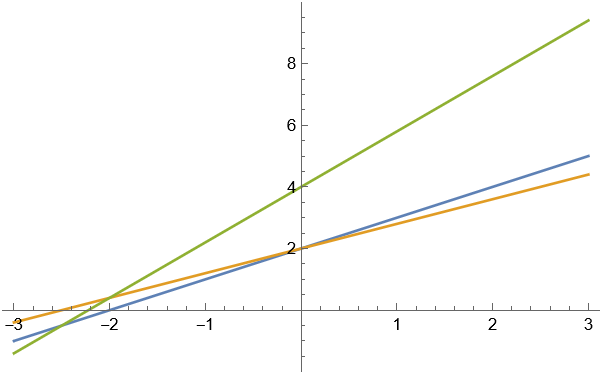
\includegraphics[width=0.4\textwidth]{Ej1c.png}\\
                    Figura 3. Suma de dos polinomios con el mismo término independiente.
                \end{center}
                Otra cuestión a considerar es el producto por escalar. Supongamos que tengo $p(x)=x+1\in S_1\to(2 p)(x)=2x+2\notin S_1$, por lo tanto, tampoco es cerrado bajo el producto por escalar.  
            \end{mdframed}
        \item Las matrices de $\R^{2\times2}$ cuya diagonal principal es nula.
            \begin{mdframed}[style=s]
                Estas matrices son de la forma 
                \begin{tightcenter}
                    $A=\begin{pmatrix}
                        0&a\\
                        b&0
                    \end{pmatrix}$
                \end{tightcenter}
                Con lo cual el conjunto en cuestión es 
                \begin{tightcenter}
                    $S=\overline{\left\{\begin{pmatrix}
                        0&1\\
                        0&0
                    \end{pmatrix}\begin{pmatrix}
                        0&0\\
                        1&0
                    \end{pmatrix}\right\}}$    
                \end{tightcenter}
                Se sabe que $\R^{2\times2}$ es un espacio vectorial. Con lo cual si se comprueban las 3 condiciones presentadas anteriormente, el conjunto de las matrices que respetan la forma de $A$ será un espacio vectorial.
                \begin{enumerate}
                    \item $\begin{pmatrix}
                            0&0\\
                            0&0
                        \end{pmatrix}\in S$ ya que $\begin{pmatrix}
                            0&0\\
                            0&0
                        \end{pmatrix}=0\cdot\begin{pmatrix}
                            0&1\\
                            0&0
                        \end{pmatrix}+0\cdot\begin{pmatrix}
                            0&0\\
                            1&0
                        \end{pmatrix}$
                    \item Sea $\alpha\in\R$ y $A\in S\to \alpha A=\alpha \begin{pmatrix}
                            0&a\\
                            b&0
                        \end{pmatrix}=\begin{pmatrix}
                            0&\alpha a\\
                            \alpha b&0
                        \end{pmatrix}\in S$
                    \item Sean $A_1,A_2\in S\to A_1+A_2=\begin{pmatrix}
                            0&a_1\\
                            b_1&0
                        \end{pmatrix}+\begin{pmatrix}
                            0&a_2\\
                            b_2&0
                        \end{pmatrix}=\begin{pmatrix}
                            0&a_1+a_2\\
                            b_1+b_2&0
                        \end{pmatrix}\in S$
                \end{enumerate}
                Por lo tanto, $S$ es un espacio vectorial.
            \end{mdframed}
        \item Las matrices de $\R^{3\times3}$ inversibles.
            \begin{mdframed}[style=s]
                Para que una matriz $A$ sea inversible, debe existir una segunda matriz $B$ tal que: $AB=BA=I$.
                \begin{enumerate}
                    \item La matriz nula no es inversible, ya que $0\cdot B=0\quad\forall B\in\R^{3\times3}$
                \end{enumerate}
                Por lo tanto, estas matrices no son un espacio vectorial.
            \end{mdframed}
    \end{enumerate}
        \item Sea GL$(3, \C) := \{A \in \C^{3\times3} : A$ es inversible$\}$. ¿Es GL$(3, \C)$ un $\C$-EV con la suma dada por $A + B = AB$ y el producto por un escalar usual?
    \begin{mdframed}[style=s]
        Uno podría pensar que se tiene el mismo incoveniente que en el último inciso del ejercicio anterior. Sin embargo, en este caso no contamos con la definición usual de la suma. Primero, voy a tratar de encontrar el elemento neutro de la suma al cual llamaré $N$. Por definición, este elemento debe cumplir:
        \begin{center}
            $N+X=X+N=X\quad\forall X\in$ GL$(3,\C)$\\
            $\to NX=XN=X$
        \end{center}
        La matriz $N$ que cumple estas propiedades es la matriz identidad. Con esto en mente me fijo si se cumplen las 3 condiciones.
        \begin{enumerate}
            \item[i.] $N=I\in$ GL$(3,\C)$ ya que la inversa de la identidad es la propia identidad.
            \item[ii.] Dadas $A,B\in$ GL$(3,\C)$, entonces existen matrices $A^*,B^*$ tales que
                $\begin{cases}
                    AA^*=A^*A=I\\
                    BB^*=B^*B=I
                \end{cases}\\\to A+B=AB$. Si considero la matriz $B^*A^*\to \begin{cases}
                    ABB^*A^*=ANA^*=AA^*=N\\
                    B^*A^*AB=B^*NB=B^*B=N
                \end{cases}$\\
                Con lo cual $A+B$ es cerrada bajo adición.
            \item[iii.] Sea $\alpha\in\C$, $X\in$ GL$(3,\C)\to \exists X^*:XX^*=X^*X=N$\\
                $\begin{cases}
                    \alpha XX^*=\alpha N=N\\
                    X^*\alpha X=\alpha X^*X=\alpha N=N
                \end{cases}\to$ es cerrada bajo producto por escalar.
        \end{enumerate}
        Por lo tanto, GL$(3,\C)$ es un $\C$-EV
    \end{mdframed}
        \item Determinar si existe $t\in\R$ tal que los vectores $(t - 1, 0, 1), (t, 1, 2)$ y $(-1, 1, -1)$ sean linealmente independientes.
    \begin{mdframed}[style=s]
        Para que los 3 vectores sean linealmente independientes, se debe cumplir que 
        \begin{center}
            $\alpha(t-1,0,1)+\beta(t,1,2)+\gamma(-1,1,-1)=\vec{0}\Leftrightarrow \alpha=\beta=\gamma=0$\\
            $\begin{cases}
                \alpha(t-1)+\beta t-\gamma=0\\
                \beta+\gamma=0\\
                \alpha+2\beta-\gamma=0
            \end{cases}\to\begin{cases}
                -3\beta(t-1)+\beta t+\beta=0\\
                \beta=-\gamma\\
                \alpha=-3\beta
            \end{cases}\to\beta(4-2t)=0$
        \end{center}
        Eligiendo $t=2$, tengo que $-3(t-1,0,1)+(t,1,2)-(-1,1,-1)=(0,0,0)$, con lo cual, los vectores son linealmente dependientes (ver Figura 4), pero si elijo cualquier otro $t$, entonces $\beta$ tiene que ser 0 y lo mismo sucede con los otros escalares. Por lo tanto, con $t\neq 2$ los vectores son li y dejan de generar sólo un plano para generar todo $\R^3$.
        \begin{center}
            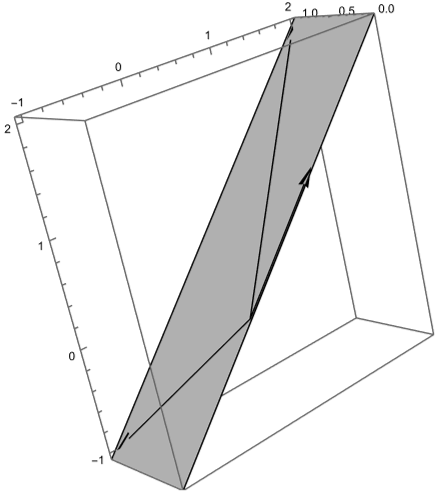
\includegraphics[width=0.28\textwidth]{Ej3.png}\\
            Figura 4. Vectores y plano que se genera con $t=2$
        \end{center}
    \end{mdframed}
        \item Demostrar que en un espacio vectorial de dimensión $n$, todo conjunto de $n+1$ vectores es linealmente dependiente.
    \begin{mdframed}[style=s]
        Llamemos al espacio $V$. Supongamos que tenemos $n$ vectores, tenemos dos opciones: que sean li o ld. Si son ld, al agregar otro vector cualquiera, el conjunto va a seguir siendo ld. Así que consideremos el caso en que tenemos un conjunto de $n$ vectores li. $B=\{b_1,\dots,b_n\}$. Al tener $n$ vectores linalmente independientes pertenecientes a un espacio de dimensión $n$, estos forman una base. Entonces cualquier $v\in V$ se escribe como combinación lineal de los $b_i,i=1,\dots,n$.\\
        Si agrego un vector cualquiera $v$ al conjunto $B$, tengo que $v=\sum_{i=1}^nx_ib_i$. Con lo cual, un conjunto de $n+1$ vectores es linealmente dependiente.
    \end{mdframed}
        \item Sea $S$ el subespacio de $\R^4$ generado por $B=\{(-1,0,-1,1);(0,1,0,-1);(-1,1,-1,0)\}$. ¿Es $B$ una base de $S$? Hallar una base de $S$ y extenderla a una de $\R^4$
    \begin{mdframed}[style=s]
        Se sabe que $S$ está generado por $B$, sin embargo, eso no me garantiza que los vectores de $B$ sean una base. Para que lo sean, deben ser li.
        \begin{center}
            $x_1(-1,0,-1,1)+x_2(0,1,0,-1)+x_3(-1,1,-1,0)=(0,0,0,0)\to \begin{cases}
                -x_1-x_3=0\\
                x_2+x_3=0\\
                -x_1-x_3=0\\
                x_1-x_2=0
            \end{cases}\to\begin{cases}
                x_1=-x_3\\
                x_2=-x_3
            \end{cases}$
        \end{center}
        Podemos elegir $x_1=x_2=-x_3=1$ y la ecuación se satisface, por ende, son ld. Me quedo con dos de estos vectores para formar una base de $S$:
        \begin{center}
            $B^*=\{(-1,0,-1,1);(0,1,0,-1)\}$
        \end{center}
        como son dos vectores y no son múltiplos, entonces son li. Para extender la base a una de $\R^4$, hay que agregar dos vectores que sean li con los de la base $B^*$, propongo $(0,0,1,0)$ y $(0,0,0,1)$. Se puede verificar que efectivamente son li y por lo tanto 
        \begin{center}
            $B_1=\{(-1,0,-1,1);(0,1,0,-1);(0,0,1,0);(0,0,0,1)\}$    
        \end{center}
        es base de $\R^4$.
    \end{mdframed}
        \item Probar que $B=\{(1,-1,-1,-1);(0,1,1,0);(1,2,0,0);(0,1,2,-1)\}$ es una base de $\C^4$ (como $\C$-EV)
    \begin{mdframed}[style=s]
        Me tengo que fijar si son li. Una forma de hacerlo es comprobar que la única manera de generar el vector nulo es con todos escalares iguales a 0.
        \begin{center}
            $z_1(1,-1,-1,-1)+z_2(0,1,1,0)+z_3(1,2,0,0)+z_4(0,1,2,-1)=(0,0,0,0)\quad z_1,z_2,z_3,z_4\in\C$
            $\begin{cases}
                z_1+z_3=0\\
                -z_1+z_2+2z_3+z_4=0\\
                -z_1+z_2+2z_4=0\\
                -z_1-z_4=0
            \end{cases}\to\begin{cases}
                z_1=-z_3\\
                z_2=-4z_3\\
                z_4=-3z_3\\
                z_4=z_3
            \end{cases}\to z_3=0\to z_1=z_2=z_4=0$
        \end{center}
        Otra manera de verificar la independencia lineal es armar una matriz cuyas columnas son los vectores en cuestión y calcular el determinante, si es cero, entonces son ld, de lo contrario son li.
        \begin{tightcenter}
            $\begin{vmatrix}
                1&0&1&0\\
                -1&1&2&1\\
                -1&1&0&2\\
                -1&0&0&-1
            \end{vmatrix}=1\begin{vmatrix}
                1&2&1\\
                1&0&2\\
                0&0&-1
            \end{vmatrix}-0\begin{vmatrix}
                -1&2&1\\
                -1&0&2\\
                -1&0&-1
            \end{vmatrix}+1\begin{vmatrix}
                -1&1&1\\
                -1&1&2\\
                -1&0&-1
            \end{vmatrix}-0\begin{vmatrix}
                -1&1&2\\
                -1&1&0\\
                -1&0&0
            \end{vmatrix}$\\
            $=1[-2(1(-1))]+1[-1(1(-1))-1(-1(-1)-2(-1))+1(-1(-1))]=2+1[1-1(1+2)+1]=2-1=1\neq 0$
        \end{tightcenter}
    \end{mdframed}
        \item Hallar una base para $\C^{2\times2}$ como $\R$-EV y como $\C$-EV. ¿Qué dimensión tiene $\C^{2\times2}$ como $\R$-EV?¿y como $\C$-EV?
    \begin{mdframed}[style=s]
        \begin{itemize}
            \item Primero vamos con el caso en que $\C^{2\times2}$ es un $\R$-EV.\\
                Sea $A\in\C^{2\times2},$
                \begin{center}
                    $A=\begin{pmatrix}
                        a&b\\
                        c&d
                    \end{pmatrix}\quad a,b,c,d\in\C$    
                \end{center}
                Para encontrar una base necesito un conjunto de matrices linealmente independiente que me generen todo $\C^{2\times2}$. Lo primero que se me ocurre es 
                \begin{center}
                    $B_1=\left\{\begin{pmatrix}
                        1&0\\0&0
                    \end{pmatrix};\begin{pmatrix}
                        0&1\\0&0
                    \end{pmatrix};\begin{pmatrix}
                        0&0\\1&0
                    \end{pmatrix};\begin{pmatrix}
                        0&0\\0&1
                    \end{pmatrix}\right\}$    
                \end{center}
                Pero como estamos considerando a $\C^{2\times2}$ como $\R$-EV, no hay manera de generar matrices con entradas complejas ya que los escalares son reales. Para subsanar este incoveniente quizás se pueda pensar en 
                \begin{center}
                    $B_2=\left\{\begin{pmatrix}
                        1+i&0\\0&0
                    \end{pmatrix};\begin{pmatrix}
                        0&1+i\\0&0
                    \end{pmatrix};\begin{pmatrix}
                        0&0\\1+i&0
                    \end{pmatrix};\begin{pmatrix}
                        0&0\\0&1+i
                    \end{pmatrix}\right\}$    
                \end{center}
                Sin embargo, otra vez tengo problemas, ya que ahora puedo tener entradas con parte real y compleja, pero no hay manera de obtener entradas con sólo parte compleja ni tampoco entradas puramente reales (la idea de estas matrices, con todas las entradas nulas excepto una, es encontrar un equivalente a una base canónica para este espacio, ya que son bastante sencillas para trabajar). Cada entrada tiene el mismo incoveniente, el de separar parte real de imaginaria. Para esto, necesito dos matrices, una con entrada real y la otra imaginaria, de esta forma puedo cubrir todos los casos. Entonces,
                \begin{center}
                    $B=\left\{\begin{pmatrix}
                        1&0\\0&0
                    \end{pmatrix};\begin{pmatrix}
                        0&1\\0&0
                    \end{pmatrix};\begin{pmatrix}
                        0&0\\1&0
                    \end{pmatrix};\begin{pmatrix}
                        0&0\\0&1
                    \end{pmatrix};\begin{pmatrix}
                        i&0\\0&0
                    \end{pmatrix};\begin{pmatrix}
                        0&i\\0&0
                    \end{pmatrix};\begin{pmatrix}
                        0&0\\i&0
                    \end{pmatrix};\begin{pmatrix}
                        0&0\\0&i
                    \end{pmatrix}\right\}$   
                \end{center}
                genera $\C^{2\times2}$ como $\R$-EV. Ahora para ver si es una base, hay que comprobar que los elementos de $B$ sean li.
                \begin{tightcenter}
                    $x_1\begin{pmatrix}
                        1&0\\0&0
                    \end{pmatrix}+x_2\begin{pmatrix}
                        0&1\\0&0
                    \end{pmatrix}+x_3\begin{pmatrix}
                        0&0\\1&0
                    \end{pmatrix}+x_4\begin{pmatrix}
                        0&0\\0&1
                    \end{pmatrix}+x_5\begin{pmatrix}
                        i&0\\0&0
                    \end{pmatrix}+x_6\begin{pmatrix}
                        0&i\\0&0
                    \end{pmatrix}+x_7\begin{pmatrix}
                        0&0\\i&0
                    \end{pmatrix}+x_8\begin{pmatrix}
                        0&0\\0&i
                    \end{pmatrix}=\begin{pmatrix}
                        0&0\\0&0
                    \end{pmatrix}\quad x_i\in\R,i=1,\dots,8$
                \end{tightcenter}
                $\begin{cases}
                    x_1+ix_5=0\\
                    x_2+ix_6=0\\
                    x_3+ix_7=0\\
                    x_4+ix_8=0
                \end{cases}\to x_1=x_2=x_3=x_4=x_5=x_6=x_7=x_8=0\to$ son li. Por lo tanto, $B$ es base.\\
                Como la base está formada por 8 elementos, dim$(\C^{2\times2})=8$ como $\R$-EV.
            \item Considerando a $C^{2\times2}$ como $\C$-EV.\\
                Vuelvo a probar 
                \begin{center}
                    $B_1=\left\{\begin{pmatrix}
                        1&0\\0&0
                    \end{pmatrix};\begin{pmatrix}
                        0&1\\0&0
                    \end{pmatrix};\begin{pmatrix}
                        0&0\\1&0
                    \end{pmatrix};\begin{pmatrix}
                        0&0\\0&1
                    \end{pmatrix}\right\}$    
                \end{center}
                Ahora ya no tengo el problema de no poder generar una matriz con entradas complejas, ya que los escalares pueden serlo. De hecho un $A\in\C^{2\times2}$ es 
                \begin{tightcenter}
                    $A=\begin{pmatrix}
                        a_{11}+ib_{11}&a_{12}+ib_{12}\\a_{21}+ib_{21}&a_{22}+ib_{22}
                    \end{pmatrix}$\\$=(a_{11}+ib_{11})\begin{pmatrix}
                        1&0\\0&0
                    \end{pmatrix}+(a_{12}+ib_{12})\begin{pmatrix}
                        0&1\\0&0
                    \end{pmatrix}+(a_{21}+ib_{21})\begin{pmatrix}
                        0&0\\1&0
                    \end{pmatrix}+(a_{22}+ib_{22})\begin{pmatrix}
                        0&0\\0&1
                    \end{pmatrix}$\\$=z_{11}\begin{pmatrix}
                        1&0\\0&0
                    \end{pmatrix}+z_{12}\begin{pmatrix}
                        0&1\\0&0
                    \end{pmatrix}+z_{21}\begin{pmatrix}
                        0&0\\1&0
                    \end{pmatrix}+z_{22}\begin{pmatrix}
                        0&0\\0&1
                    \end{pmatrix}\quad z_{11},z_{12},z_{21},z_{22}\in\C$
                \end{tightcenter}
                Por lo tanto, los elementos de $B_1$ generan $\C^{2\times2}$ y como además se ve que son li, $B$ es base. Al tener 4 elementos, dim$(\C^{2\times2})=4$ como $\C$-EV.
        \end{itemize}
    \end{mdframed}
        \item Analizar en cada caso si el conjunto el linealmente independiente y hallar el subespacio generado por cada uno de ellos. Decir además qué dimensión tiene cada subespacio.
    \begin{enumerate}
        \item $B=\{(2,0,1);(3,1,2);(1,1,1);(7,3,5)\}\subset\R^3$
            \begin{mdframed}[style=s]
                Del ejercicio 4, se deduce que $B$ es un conjunto linealmente dependiente. Sea $v\in B$
                \begin{center}
                    $v=x_1(2,0,1)+x_2(3,1,2)+x_3(1,1,1)+x_4(7,3,5)\quad x_1,x_2,x_3,x_4\in\R$\\
                    $v=(2x_1+3x_2+x_3+7x_4,x_2+x_3+3x_4,x_1+2x_2+x_3+5x_4)$\\
                \end{center}
                Manipulando la expresión:
                \begin{center}
                    $v=(x_2+x_3+3x_4)(1,1,1)+(x_1+x_2+2x_4)(2,0,1)$
                \end{center}
                Se puede ver que $v$ es una combinación lineal de $(1,1,1)$ y $(2,0,1)$. En la Figura 5, se pueden observar los 4 vectores de $B$ y el plano en el que están contenidos
                \begin{center}
                    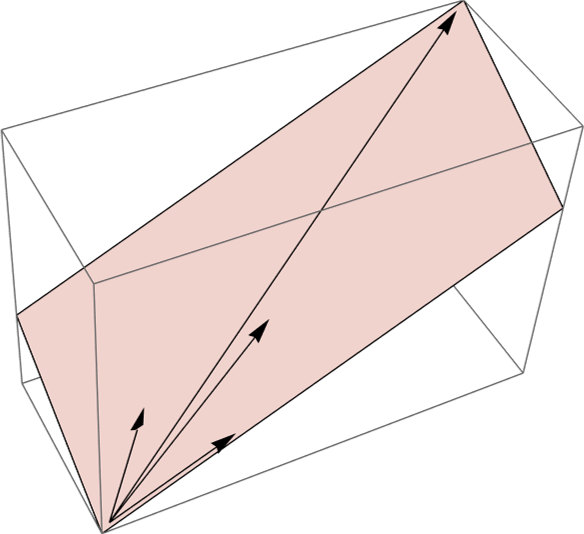
\includegraphics[width=0.4\textwidth]{Ej8.png}\\
                    Figura 5. Espacio generado por un conjunto de vectores.
                \end{center}
                El plano que generan se puede encontrar haciendo el producto vectorial entre los vectores generadores y se obtiene $\pi:x+y-2z=0$. Como generan un plano, la dimensión del espacio generado es 2.
            \end{mdframed}
        \item $B=\left\{\begin{pmatrix}
                2&1\\0&0
            \end{pmatrix};\begin{pmatrix}
                0&0\\2&1
            \end{pmatrix};\begin{pmatrix}
                3&-1\\0&0
            \end{pmatrix}\right\}\subset\R^{2\times2}$
            \begin{mdframed}[style=s]
                $x_1\begin{pmatrix}
                    2&1\\0&0
                \end{pmatrix}+x_2\begin{pmatrix}
                    0&0\\2&1
                \end{pmatrix}+x_3\begin{pmatrix}
                    3&-1\\0&0
                \end{pmatrix}=\begin{pmatrix}
                    0&0\\0&0
                \end{pmatrix}\to \begin{cases}
                    2x_1+3x_3=0\\
                    x_1-x_3=0\\
                    2x_2=0\\
                    x_2=0
                \end{cases}\to x_1=x_2=x_3=0$\\
                Por lo tanto, $B$ es un conjunto linealmente independiente, entonces
                \begin{center}
                    $\overline{B}=\overline{\left\{\begin{pmatrix}
                        2&1\\0&0
                    \end{pmatrix};\begin{pmatrix}
                        0&0\\2&1
                    \end{pmatrix};\begin{pmatrix}
                        3&-1\\0&0
                    \end{pmatrix}\right\}}$.
                \end{center}
                También se puede pensar en que el espacio generado está compuesto por matrices de la forma
                \begin{center}
                    $A=\begin{pmatrix}
                        a&b\\2d&d
                    \end{pmatrix}\quad a,b,d\in\R$
                \end{center}
                Es decir, 
                \begin{center}
                    $\overline{B}=\left\{\begin{pmatrix}
                        a_{11}&a_{12}\\a_{21}&a_{22}
                    \end{pmatrix}\in\R^{2\times2}:2a_{22}=a_{21}\right\}$    
                \end{center}
                Por último, dim$(\overline{B})=3$
            \end{mdframed}
        \item $B=\{1-x,2-x^2,x+x^2\}\subset\R_2[x]$ (el conjunto de polinomios de grado menor o igual a 2 con coeficientes en $\R$).
            \begin{mdframed}[style=s]
                \begin{center}
                    $\alpha(1-x)+\beta(2-x^2)+\gamma(x+x^2)=0\to\begin{cases}
                        \alpha+2\beta=0\\
                        -\alpha+\gamma=0\\
                        -\beta+\gamma=0
                    \end{cases}\to \alpha=\beta=\gamma=0\to$ son li.
                \end{center}
                Como son 3 polinomios li de un espacio de dimensión 3, generan a $\R_2[x]$.
            \end{mdframed}
    \end{enumerate}
    
        \item Sea $B=\{x^k:k\in\mathbb{N}\}\subset\C[x]$
    \begin{enumerate}
        \item Probar que todo subconjunto finito de $B$ es linealmente independiente.
            \begin{mdframed}[style=s]
                Un subconjunto $A$ de $B$ será de la forma: 
                \begin{center}
                    $A=\{x^{k_1},x^{k_2},\dots,x^{k_n}\}\quad k_i\neq k_j,\forall j\neq i\quad i,j=1,\dots,n$    
                \end{center}
                Para saber si son li, tengo que verificar que la única solución a 
                \begin{equation}
                    \sum_{i=1}^n\alpha_ix^{k_i}=0,\quad \alpha_i\in\C
                \end{equation}
                sea la trivial. Se puede reescribir al polinomio nulo como
                \begin{equation*}
                    0=\sum_{i=1}^n0\cdot x^{k_i}
                \end{equation*}
                Se ve que el polinomio nulo tiene coeficiente 0 para toda potencia de $x$ y como los elementos de $A$ tienen todos exponentes diferentes, la única manera que (1) sea cierta es si $\alpha_i=0\quad\forall i$, por ende, $A$ es un conjunto linealmente independiente.
            \end{mdframed}
        \item ¿Es $B$ una base de $\C[x]$ como $\C$-EV?
            \begin{mdframed}[style=s]
                En el inciso anterior, se vio que todo subconjunto de $B$ es linealmente independiente. En particular, $B$ es un subconjunto de si mismo, con lo cual $B$ es li. Resta ver que genere a $\C[x]$. Dado un $p\in\C[x]$, éste puede escribirse como 
                \begin{equation*}
                    p(x)=\sum_{i=1}^n\alpha_ix^{k_i}\quad \alpha_i\in\C,\forall i
                \end{equation*}
                Que es exactamente una combinación lineal de los elementos de $B$, entonces $B$ genera $\C[x]$. Por lo tanto, es base.
            \end{mdframed}
        \item ¿Cuál es la dimensión de $\C[x]$ como $\C$-EV?
            \begin{mdframed}[style=s]
                La dimensión del espacio está determinada por la cantidad de elementos de una base, en este caso $B$ tiene $n$ elementos, este número natural puede ser tan grande como quiera, entonces $dim(\C[x])=\infty$
            \end{mdframed}
    \end{enumerate}
        \item Sea $V$ un $\mathbb{K}$-EV de dimensión finita y $U$ un subespacio de $V$. Probar que, si la dimensión de $U$ coincide con la de $V$ entonces $U=V$.
    \begin{mdframed}[style=s]
        Dada una base $B$ de $U$, está tendrá $n$ elementos si la $dim(U)=dim(V)=n$. Como $U$ es subespacio, $B$ también es li en $V$ y por ende será una base de $V$, entonces como $U$ y $V$ tienen la misma base, son el mismo espacio.
    \end{mdframed}
        \item Sean $W_1$ y $W_2$ subespacios de un espacio vectorial $V$ ¿Son $W_1\cap W_2$ y $W_1\cup W_2$ subespacios de $V$?. Justificar.
    \begin{mdframed}[style=s]
        Dado $s_1,s_2\in W_1\cap W_2, \lambda\in\mathbb{K}$
        \begin{enumerate}
            \item[i.] $\vec{0}\in W_1\cap W_2$ ya que $\vec{0}\in W_1, \vec{0}\in W_2$ por ser subespacios.
            \item[ii.] $\begin{cases}
                    s_1+s_2\in W_1 \text{ ya que } s_1\in W_1,s_2\in W_1\\
                    s_1+s_2\in W_2 \text{ ya que } s_1\in W_2,s_2\in W_2
                \end{cases}\to s_1+s_2\in W_1\cap W_2$
            \item[iii.] $\begin{cases}
                    \lambda s_1\in W_1 \text{ ya que } s_1\in W_1,\\
                    \lambda s_1\in W_2 \text{ ya que } s_1\in W_2
                \end{cases}\to \lambda s_1\in W_1\cap W_2$
        \end{enumerate}
        Se concluye que $W_1\cap W_2$ es un subespacio de $V$.\\
        En el caso de la unión no sucede lo mismo.\\
        Supongamos que 
        \begin{tightcenter}
            $V=\R^2,W_1=\{(x,y)\in\R^2:y=0\},W_2=\{(x,y)\in\R^2:x=0\}$    
        \end{tightcenter}
        Ahora sean 
        \begin{tightcenter}
            $v_1=(1,0)\in W_1\cup W_2, v_2=(0,1)\in W_1\cup W_2$    
        \end{tightcenter}
        se tiene que 
        \begin{tightcenter}
            $v_1+v_2=(1,1)\notin W_1\cup W_2$    
        \end{tightcenter}
        Entonces, la unión no es cerrada bajo adición. Por lo tanto, no es un subespacio.
    \end{mdframed}
        \item Probar que $W_1+W_2=\overline{W_1\cup W_2}$ y, por lo tanto, $W_1+W_2$ es un subespacio de $V$.
    \begin{mdframed}[style=s]
        \begin{enumerate}
            \item[i.] Dado $s\in W_1+W_2\to s=w_1+w_2, w_1\in W_1,w_2\in W_2\to s\in \overline{W_1\cup W_2}\to W_1+W_2\subset\overline{W_1\cup W_2}$.
            \item[ii.] Dado $s\in\overline{W_1\cup W_2}\to s=\alpha w_1+\beta w_2,\alpha,\beta\in\mathbb{K},w_1\in W_1,w_2\in W_2$, como $W_1,W_2$ son subespacios $\alpha w_1\in W_1, \beta w_2\in W_2\to s=b_1+b_2, b_1\in W_1,b_2\in W_2\to s\in W_1+W_2\to\overline{W_1\cup W_2}\subset W_1+W_2$.
        \end{enumerate}
        De i. y ii. se tiene que
        \begin{tightcenter}
            $\overline{W_1\cup W_2}=W_1+W_2$
        \end{tightcenter}
        Para que de esa igualdad se concluya que $W_1+W_2$ es un subespacio tendría que haber probado antes que $\overline{W_1\cup W_2}$ es un subespacio, cosa que no sucedió. Voy a probar del modo convencional:
        \begin{enumerate}
            \item[i.] $0\in W_1+W_2$ ya que $0=0+0,0\in W_1,0\in W_2$
            \item[ii.] Dados $s,t\in W_1+W_2\to s+t=s_1+s_2+t_1+t_2,\quad s_1,t_1\in W_1, s_2,t_2\in W_2\to s+t=s_1+t_1+s_2+t_2$. Como $W_1,W_2$ son subespacios \\
                $a_1=s_1+t_1\in W_1, a_2=s_2+t_2\in W_2\to s+t=a_1+a_2,\quad a_1\in W_1, a_2\in W_2\to s+t\in W_1+W_2$ 
            \item[iii.] Sea $\alpha\in\mathbb{K},s\in W_1+W_2\to \alpha s=\alpha(s_1+s_2),\quad s_1\in W_1,s_2\in W_2\to s=\alpha s_1+\alpha s_2,\quad \alpha s_1\in W_1, \alpha s_2\in W_2\to\alpha s\in W_1+W_2$
        \end{enumerate}
        Por lo tanto, $W_1+W_2$ es un subespacio de $V$.
    \end{mdframed}
        \item Sean $V_1=\{A\in\C^{2\times2}:a_{11}+a_{12}=0\}$ y $V_2=\{A\in\C^{2\times2}:a_{11}+a_{21}=0\}$
    \begin{enumerate}
        \item Probar que $V_1$ y $V_2$ son subespacios de $\C^{2\times2}$ (como $\C$-EV).
            \begin{mdframed}[style=s]
                \begin{itemize}
                    \item $V_1$:
                    \begin{enumerate}
                        \item $\begin{pmatrix}
                                0&0\\0&0
                            \end{pmatrix}\in V_1$ ya que $0+0=0$
                            \item Sean $A,B\in V_1$ 
                                \begin{center}
                                    $\to A+B=\begin{pmatrix}
                                        a_{11}&a_{12}\\a_{21}&a_{22}
                                    \end{pmatrix}+\begin{pmatrix}
                                        b_{11}&b_{12}\\b_{21}&b_{22}
                                    \end{pmatrix}=\begin{pmatrix}
                                        a_{11}+b_{11}&a_{12}+b_{12}\\a_{21}+b_{21}&a_{22}+b_{22}
                                    \end{pmatrix}$    
                                \end{center}
                                Y como $a_{11}+b_{11}+a_{12}+b_{12}=a_{11}+a_{12}+b_{11}+b_{12}=0+0=0\to A+B\in V_1$
                            \item Sea $\alpha\in\C, A\in V_1$
                                \begin{center}
                                    $\to\alpha A=\alpha\begin{pmatrix}
                                        a_{11}&a_{12}\\a_{21}&a_{22}
                                    \end{pmatrix}=\begin{pmatrix}
                                        \alpha a_{11}&\alpha a_{12}\\\alpha a_{21}&\alpha a_{22}
                                    \end{pmatrix}$    
                                \end{center}
                                de donde $\alpha a_{11}+\alpha a_{12}=\alpha(a_{11}+a_{12})=\alpha 0=0\to \alpha A\in V_1$
                        \end{enumerate}
                        Entonces, $V_1$ es subespacio de $\C^{2\times2}$
                    \item $V_2:$\\
                        La demostración es análoga a la anterior cambiando las entradas 12 por la 21.
                \end{itemize}
            \end{mdframed}
        \item Hallar $V_1\cap V_2$ y $V_1+V_2$.
            \begin{mdframed}[style=s]
                \begin{itemize}
                    \item $V_1\cap V_2=\{A\in\C^{2\times2}:a_{11}+a_{12}=0,a_{11}+a_{21}=0\}=\left\{A\in\C^{2\times2}:A=\begin{pmatrix}
                            a_{11}&-a_{11}\\-a_{11}&a_{22}    
                        \end{pmatrix}\right\}$
                        \begin{center}
                            $\to A=\overline{\left\{\begin{pmatrix}
                                1&-1\\-1&0
                            \end{pmatrix};\begin{pmatrix}
                                0&0\\0&1
                            \end{pmatrix}\right\}}$
                        \end{center}
                    \item $V_1+V_2=\{A\in\C^{2\times2}:A=X+Y,\quad X\in V_1,Y\in V_2\}$\\
                        Entonces, tengo que 
                        \begin{center}
                            $A=\begin{pmatrix}
                                x_{11}&-x_{11}\\x_{21}&x_{22}
                            \end{pmatrix}+\begin{pmatrix}
                                y_{11}&y_{12}\\-y_{11}&y_{22}
                            \end{pmatrix}=\begin{pmatrix}
                                x_{11}+y_{11}&-x_{11}+y_{12}\\x_{21}-y_{11}&x_{22}+y_{22}
                            \end{pmatrix}$    
                        \end{center}
                        Por lo tanto, $A$ es una combinación lineal de
                        \begin{center}
                            $A=x_{11}\begin{pmatrix}
                                1&-1\\0&0
                            \end{pmatrix}+x_{21}\begin{pmatrix}
                                0&0\\1&0
                            \end{pmatrix}+x_{22}\begin{pmatrix}
                                0&0\\0&1
                            \end{pmatrix}+y_{11}\begin{pmatrix}
                                1&0\\-1&0
                            \end{pmatrix}+y_{12}\begin{pmatrix}
                                0&1\\0&0
                            \end{pmatrix}+y_{22}\begin{pmatrix}
                                0&0\\0&1
                            \end{pmatrix}$\\
                            $A=x_{11}\begin{pmatrix}
                                1&-1\\0&0
                            \end{pmatrix}+x_{21}\begin{pmatrix}
                                0&0\\1&0
                            \end{pmatrix}+(x_{22}+y_{22})\begin{pmatrix}
                                0&0\\0&1
                            \end{pmatrix}+y_{11}\begin{pmatrix}
                                1&0\\-1&0
                            \end{pmatrix}+y_{12}\begin{pmatrix}
                                0&1\\0&0
                            \end{pmatrix}$
                        \end{center}
                        Se ve que la matriz que tiene como coeficiente a $x_{11}$ es una combinación lineal de las matrices cuyos coeficientes son $x_{21},y_{11}$ y $y_{12}$
                        \begin{center}
                            $\begin{pmatrix}
                                1&-1\\0&0
                            \end{pmatrix}=\begin{pmatrix}
                                0&0\\1&0
                            \end{pmatrix}+\begin{pmatrix}
                                1&0\\-1&0
                            \end{pmatrix}-\begin{pmatrix}
                                0&1\\0&0
                            \end{pmatrix}$
                        \end{center}
                        Entonces, se tiene que
                        \begin{center}
                            $A=x_{21}\begin{pmatrix}
                                0&0\\1&0
                            \end{pmatrix}+(x_{22}+y_{22})\begin{pmatrix}
                                0&0\\0&1
                            \end{pmatrix}+y_{11}\begin{pmatrix}
                                1&0\\-1&0
                            \end{pmatrix}+y_{12}\begin{pmatrix}
                                0&1\\0&0
                            \end{pmatrix}$
                        \end{center}
                    Estas 4 matrices son li, con lo que se concluye que una base de $V_1+V_2$ es 
                    \begin{center}
                        $B=\left\{\begin{pmatrix}
                            0&0\\1&0
                        \end{pmatrix};\begin{pmatrix}
                            0&0\\0&1
                        \end{pmatrix};\begin{pmatrix}
                            1&0\\-1&0
                        \end{pmatrix};\begin{pmatrix}
                            0&1\\0&0
                        \end{pmatrix}\right\}$    
                    \end{center}
                    Al tener 4 elementos, el subespacio es de dimensión 4. Entonces, 
                    \begin{center}
                        $V_1+V_2=\C^{2\times2}$    
                    \end{center}
                \end{itemize}
            \end{mdframed}
        \item Hallar las dimensiones de $V_1,V_2, V_1\cap V_2$ y $V_1+V_2$
            \begin{mdframed}[style=s]
                \begin{itemize}
                    \item Sea $A\in V_1$
                        \begin{center}
                            $\to A=\begin{pmatrix}
                                a_{11}&-a_{11}\\a_{21}&a_{22}
                            \end{pmatrix}=a_{11}\begin{pmatrix}
                                1&-1\\0&0
                            \end{pmatrix}+a_{21}\begin{pmatrix}
                                0&0\\1&0
                            \end{pmatrix}+a_{22}\begin{pmatrix}
                                0&0\\0&1
                            \end{pmatrix}$        
                        \end{center}
                        $A$ es combinación lineal de 3 matrices li, entonces $dim(V_1)=3$
                    \item Sea $A\in V_2$
                        \begin{center}
                            $\to A=\begin{pmatrix}
                                a_{11}&a_{12}\\-a_{11}&a_{22}
                            \end{pmatrix}=a_{11}\begin{pmatrix}
                                1&0\\-1&0
                            \end{pmatrix}+a_{21}\begin{pmatrix}
                                0&1\\0&0
                            \end{pmatrix}+a_{22}\begin{pmatrix}
                                0&0\\0&1
                            \end{pmatrix}$        
                        \end{center}
                        $A$ es combinación lineal de 3 matrices li, entonces $dim(V_2)=3$
                    \item Del inciso anterior se ve que $V_1\cap V_2$ está generado por 2 matrices li. Entonces $dim(V_1\cap V_2)=2$
                    \item $V_1+V_2=\C^{2\times2}\to dim(V_1+V_2)=4$
                \end{itemize}
            \end{mdframed}
    \end{enumerate}
        \item Sea $S=\{(x,y,z):x-y+z=0\}$.
    \begin{enumerate}
        \item Probar que $S$ es un subespacio de $\R^3$ y hallar una base para $S$.
            \begin{mdframed}[style=s]
                \begin{enumerate}
                    \item El vector $(0,0,0)\in S$ ya que $0-0+0=0$
                    \item Sean $s_1=(x_1,y_1,z_1),s_2=(x_2,y_2,z_2)\in S$\\
                        $\to s_1+s_2=(x_1,y_1,z_1)+(x_2,y_2,z_2)=(x_1+x_2,y_1+y_2,z_1+z_2)$\\
                        De donde, $x_1+x_2-(y_1-y_2)+z_1+z_2=x_1-y_1+z_1+x_2-y_2+z_2=0+0=0\to s_1+s_2\in S$
                    \item Sea $\alpha\in\R,s\in S\to \alpha s=\alpha(x,y,z)=(\alpha x, \alpha y,\alpha z)$\\
                        $\to \alpha x -\alpha y+\alpha z=\alpha(x-y+z)=\alpha 0=0\to\alpha s\in S$
                \end{enumerate}
                Por ende, $S$ es subespacio de $\R^3$\\
                Cualquier elemento de $S$ cumple con $x-y+z=0\to$ sea un $s\in S,s=(y-z,y,z)=y(1,1,0)+z(-1,0,1)$. Como un vector arbitrario de $S$ es combinación lineal de $(1,1,0);(-1,0,1)$, los cuales son li, $B=\{(1,1,0);(-1,0,1)\}$ es una base de $S$. En la Figura 6 se observa el plano $x-y+z=0$, y los dos vectores de la base.
                \begin{center}
                    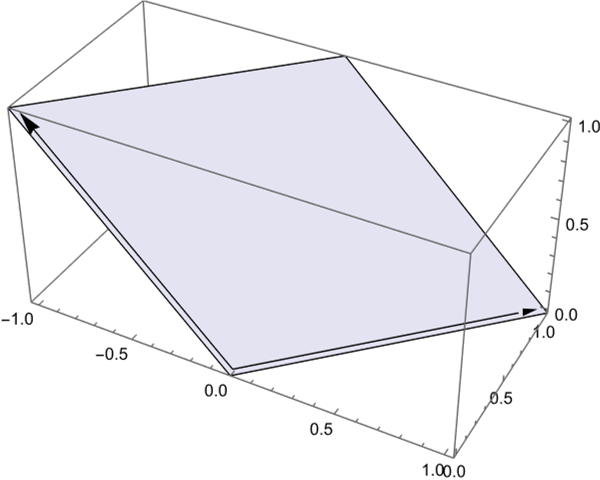
\includegraphics[width=0.4\textwidth]{Ej14.png}\\
                    Figura 6. Plano $x-y+z=0$ con vectores de la base.
                \end{center}
            \end{mdframed}
        \item Hallar un subespacio $T$ de $\R^3$ tal que $S+T=\R^3$¿Es único?
            \begin{mdframed}[style=s]
                Quiero un subespacio que al sumarlo con el plano del inciso anterior obtenga $\R^3$. Lo primero que se me ocurre es en una recta que corte al plano en un único punto y contenga al origen. Al sumar los vectores de esta recta con los del plano me puedo desplazar por todo $\R^3$. Las rectas más sencillas son los ejes coordenados.\\
                En el caso del eje de abscisas, tenemos que $T=\overline{\{(1,0,0)\}}$. Para comprobar que la suma sea realmente $\R^3$ tomemos un vector $v=(x,y,z)$ de $\R^3$. 
                \begin{center}
                    $(x,y,z)=\alpha(1,1,0)+\beta(-1,0,1)+\gamma(1,0,0)$\\
                    $\begin{cases}
                        x=\alpha-\beta+\gamma\\
                        y=\alpha\\
                        z=\beta
                    \end{cases}\to\begin{cases}
                        \gamma=x-y+z
                    \end{cases}$\\
                    $\to v=y(1,1,0)+z(-1,0,1)+(x-y+z)(1,0,0)$
                \end{center}
                Con esto se ve que cualquier vector de $\R^3$ puede ser escrito como la suma de un vector de $S$(en este caso $s=y(1,1,0)+z(-1,0,1)$) y otro de $T$($t=(x-y+z)(1,0,0)$). En la Figura 7 se muestra un caso en particular de esta situación:
                \begin{center}
                    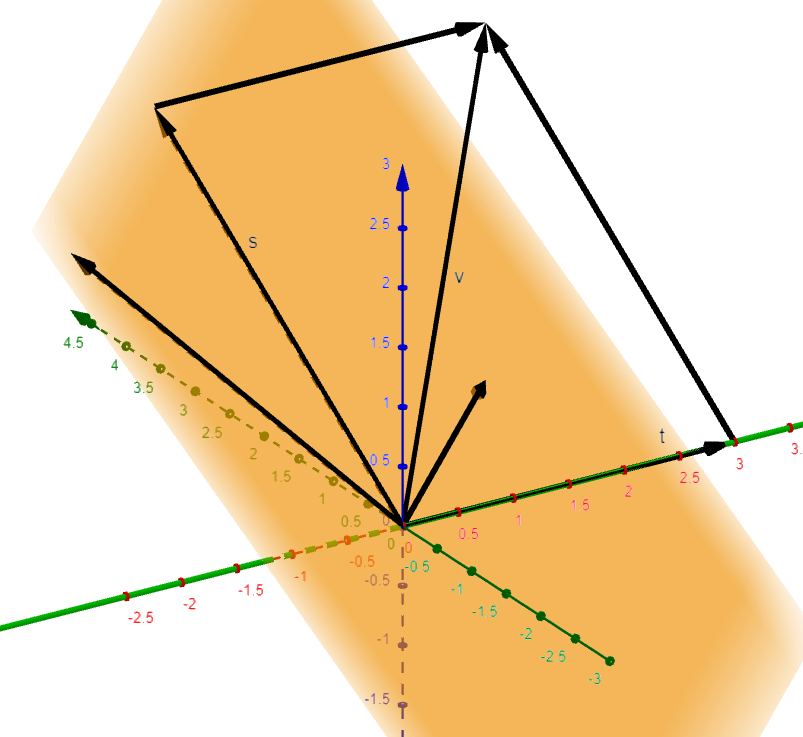
\includegraphics[width=0.4\textwidth]{Ej14b.png}\\
                    Figura 7. $v=(2,2,3)$ como combinación lineal de $s=(2,2,0)+(-3,0,3)$ y $t=(3,0,0)$
                \end{center}
                Un argumento análogo se puede hacer con cualquiera de las rectas mencionadas. ¿Qué sucede con los planos?\\
                Supongamos un plano cualquiera que contenga al origen $\pi:\alpha x+\beta y+\gamma z=0$. Los vectores de dicho plano se pueden escribir como $t=(\frac{-\beta y-\gamma z}{\alpha},y,z)=y(\frac{-\beta}{\alpha},1,0)+z(\frac{-\gamma}{\alpha},0,1)$. Por lo tanto, un elemento $v\in S+T$, siendo $T$ el plano $\pi$ se puede escribir como $v=s+t,\quad s\in S,t\in T$
                \begin{center}
                    $v=(x,y,z)=a(1,1,0)+b(-1,0,1)+c(\frac{-\beta}{\alpha},1,0)+d(\frac{-\gamma}{\alpha},0,1)$\\
                \end{center}
                \begin{itemize}
                    \item Si por ejemplo, $\pi$ fuese el plano $x-y+z=0$, tenemos que $S=T$
                        \begin{center}
                            $\to v=(x,y,z)=a(1,1,0)+b(-1,0,1)+c(1,1,0)+d(-1,0,1)$\\
                            $\to v=(a+c)(1,1,0)+(b+d)(-1,0,1)$
                        \end{center}
                        Osea que los $v$ son generados por dos vectores, entonces $S+T=S$ como era de esperarse.
                    \item En el caso que tenga otro plano $\frac{-\beta}{\alpha}=\lambda\neq 1$.
                        \begin{center}
                            $\to v=(x,y,z)=a(1,1,0)+b(-1,0,1)+c(\lambda,1,0)+d(\epsilon,0,1)$
                        \end{center}
                        Se puede comprobar que $(\epsilon,0,1)=\frac{\epsilon+1}{1-\lambda}(1,1,0)+(-1,0,1)-\frac{\epsilon+1}{1-\lambda}(\lambda,1,0)$
                        \begin{center}
                            $\to v=(x,y,z)=a(1,1,0)+b(-1,0,1)+c(\lambda,1,0)$
                        \end{center}
                        $v$ se escribe como combinación lineal de 3 vectores li (ya que $\lambda\neq -1$), entonces, una base de $S+T$ es $B=\{(1,1,0);(-1,0,1);(\lambda,1,0)\}$. Como la base tiene 3 elementos, $dim(S+T)=3$ y como es subespacio de $\R^3\to S+T=\R^3$.\\
                        También podría haber puesto la condición $\frac{-\beta}{\gamma}=\epsilon\neq -1$ y hubiese llegado a un resultado similar.
                    \item Como último caso, propongo que $T=\R^3$, entonces tendría que un $v\in S+T$ se escribe
                        \begin{center}
                            $v=(x,y,z)=a(1,1,0)+b(-1,0,1)+c(1,0,0)+d(0,1,0)+e(0,0,1)$\\
                            $\to v=c(1,0,0)+d(0,1,0)+e(0,0,1)$
                        \end{center}
                        Por lo tanto, $S+T=\R^3$.
                \end{itemize}
                
            \end{mdframed}
    \end{enumerate}
        \item Hallar una base de $V_1+V_2+V_3$ para los siguientes subespacios de $\R^5$.
    \begin{enumerate}
        \item $V_1=\overline{(1,1,2,0,1);(2,0,3,0,1)}, V_2=\overline{(-1,1,-2,1,1)}$ y $V_3=\overline{(0,1,0,1,1)}$.
            \begin{mdframed}[style=s]
                Sea $v\in V_1+V_2+V_3,v=v_1+v_2+v_3\quad v_1\in V_1,v_2\in V_2,v_3\in V_3$. Además, tenemos que
                \begin{center}
                    $v_1=a(1,1,2,0,1)+b(2,0,3,0,1)\quad a,b\in\R$\\
                    $v_2=c(-1,1,-2,1,1)\quad c\in\R$\\
                    $v_3=d(0,1,0,1,1)\quad d\in\R$
                \end{center}
                Por lo tanto,
                \begin{center}
                    $v=a(1,1,2,0,1)+b(2,0,3,0,1)+c(-1,1,-2,1,1)+d(0,1,0,1,1)\quad a,b,c,d\in\R$
                \end{center}
                Tenemos que $V_1+V_2+V_3=\overline{\{(1,1,2,0,1);(2,0,3,0,1);(-1,1,-2,1,1);(0,1,0,1,1)\}}$. Se puede comprobar que los vectores son li, entonces una posible base es
                \begin{center}
                    $B=\{(1,1,2,0,1);(2,0,3,0,1);(-1,1,-2,1,1);(0,1,0,1,1)\}$
                \end{center}
            \end{mdframed}
        \item $V_1=\overline{(1,1,2,0,1);(2,0,3,0,1)}, V_2=\overline{(1,0,-2,1,1)}$ y $V_3=\overline{(1,1,1,2,2)}$.
            \begin{mdframed}[style=s]
                Es un caso análogo al anterior, y se puede llegar a que una posible base entonces
                \begin{center}
                    $B=\{(1,1,2,0,1);(2,0,3,0,1);(1,0,-2,1,1);(1,1,1,2,2)\}$
                \end{center}
            \end{mdframed}
    \end{enumerate}
        \item Sea $C(\R)$ el $\R$-EV de las funciones continuas de $\R$ en $\R$, con las operaciones usuales. Si $V\subset C(\R)$ es el conjunto de funciones pares y $W\subset C(\R)$ el de las impares, probar que:
    \begin{enumerate}
        \item $V$ y $W$ son subespacios de $C(\R)$.
            \begin{mdframed}[style=s]
                \begin{itemize}
                    \item $V=\{f\in C(\R):f(x)=f(-x)\quad\forall x\in\R\}$
                        \begin{enumerate}
                            \item $f(x)=0\in V$ ya que $f(x)=f(-x)=0$
                            \item Sean $f_1,f_2\in V\to (f_1+f_2)(x)=f_1(x)+f_2(x)=f_1(-x)+f_2(-x)=(f_1+f_2)(-x)\to f_1+f_2\in V$
                            \item Sean $\alpha\in\R,f\in V\to (\alpha f)(x)=\alpha f(x)=\alpha f(-x)=(\alpha f)(-x)\to\alpha f\in V$
                        \end{enumerate}
                        Se concluye que $V$ es subespacio.
                    \item $W=\{f\in C(\R):f(-x)=-f(x)\quad\forall x\in\R\}$
                        \begin{enumerate}
                            \item $f(x)=0\in V$ ya que $f(-x)=-f(x)=0$
                            \item Sean $f_1,f_2\in V\to (f_1+f_2)(-x)=f_1(-x)+f_2(-x)=-f_1(x)-f_2(x)=-(f_1+f_2)(x)\to f_1+f_2\in V$
                            \item Sean $\alpha\in\R,f\in V\to (\alpha f)(-x)=\alpha f(-x)=-\alpha f(x)=-(\alpha f)(x)\to\alpha f\in V$
                        \end{enumerate}
                        Se concluye que $W$ es subespacio.
                \end{itemize}
            \end{mdframed}
        \item $V\cap W=\{0\}$.
            \begin{mdframed}[style=s]
                La intersección estará formada funciones que sean pares e impares a la vez. Es decir, tienen que satisfacer
                \begin{enumerate}
                    \item $f(x)=f(-x)$
                    \item $f(-x)=-f(x)$
                \end{enumerate}
                Entonces, $f(x)=-f(x)\to f(x)=0\to V\cap W=\{0\}$
            \end{mdframed}
        \item $V+W=C(\R)$.
            \begin{mdframed}[style=s]
                Implica que toda función continua puede ser escrita como la suma de una función par y otra impar.\\
                Como $V$ y $W$ son subespacios, $V+W$ también lo es.\\
                \textbf{Completar.}
            \end{mdframed}
    \end{enumerate}
        \item Sean $W_1$ y $W_2$ subespacios de un espacio vectorial $V$ tales que, $W_1\cap W_2=\{0\}$ y $V=W_1+W_2$. Probar que, dado $v\in V$, existen únicos $w_1\in W_1$ y $w_2\in W_2$ tales que $v=w_1+w_2$
    \begin{mdframed}[style=s]
        Supongamos las bases $B_1=\{v_1,\dots,v_m\}, B_2=\{v_{m+1},\dots,v_n\}$ de $W_1$ y $W_2$ respectivamente. Dado un $v\in V$, este puede ser escrito como
        \begin{center}
            $v=w_1+w_2, \quad w_1\in W_1,w_2\in W_2$
        \end{center}
        debido a que $V=W_1+W_2$. Por lo tanto,
        \begin{center}
            $v=x_1v_1+\dots+x_mv_m+x_{m+1}v_{m+1}+\dots+x_nv_n$
        \end{center}
        Si $v$ se pudiese escribir como la suma de otros dos vectores, tenemos la siguiente situación
        \begin{center}
            $v=y_1v_1+\dots+y_mv_m+y_{m+1}v_{m+1}+\dots+y_nv_n$
        \end{center}
        Restando ambas igualdades obtenemos
        \begin{center}
            $0=(x_1-y_1)v_1+\dots+(x_m-y_m)v_m+(x_{m+1}-y_{m+1})v_{m+1}+\dots+(x_n-y_n)v_n$
        \end{center}
        Como $W_1\cap W_2=\{0\}\to$ los $v_i,i=1,\dots,n$ son vectores li y forman una base de $V$, entonces por definición de independencia lineal
        \begin{equation*}
            \sum_{i=1}^n(x_i-y_i)v_i=0\Leftrightarrow(x_i-y_i)=0\quad\forall i=1,\dots,n
        \end{equation*}
        Por lo tanto,
        \begin{center}
            $x_i=y_i\quad\forall i=1,\dots,n$
        \end{center}
        Lo que implica que $v$ se puede escribir de manera única.\vspace{6pt}\\
        A modo de ejemplo, se puede pensar en $V=\R^2,W_1=\{(x,y)\in\R^2:y=0\},W_2=\{(x,y)\in\R^2:x=0\}$. Si quisiese representar al $(1,1)$ es claro que la única manera es con el $(1,0)$ y el $(0,1)$.
    \end{mdframed}
    \end{enumerate}
\end{document}